\documentclass[tikz, border=0pt]{standalone}
\usepackage{tikz}
\tikzset{
	>=latex
}
\usepackage[utf8]{inputenc}
\usepackage[T1]{fontenc}
\usepackage{mathpazo}
\usepackage[scaled]{beramono}
\usetikzlibrary{arrows.meta}
\usetikzlibrary{calc}
\usetikzlibrary{spy}
\usepackage{pgfplots}
\pgfplotsset{compat=1.13}
\usepackage[outline]{contour}
\contourlength{1.2pt}

\begin{document}
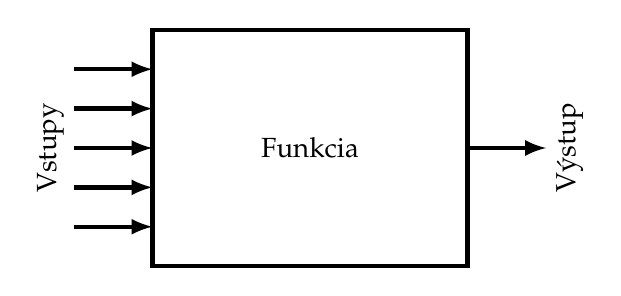
\begin{tikzpicture}
	%\draw[help lines] (0,0) grid (14,10);

	\draw[ultra thick] (4,3) rectangle (8,6);

	\foreach \y in {3.5,4,...,5.5}{
		\draw[ultra thick, latex-] (4,\y) -- ++(-1,0);
	}
	\draw[ultra thick, -latex] (8,4.5) -- ++(1,0);

	\draw (3,4.5) node[anchor=east]{\rotatebox{90}{Vstupy}};
	\draw (9,4.5) node[anchor=west]{\rotatebox{90}{Výstup}};
	\draw (6,4.5) node{\rotatebox{0}{Funkcia}};

\end{tikzpicture}
\end{document}
